% Report Reflection Amplifier Rev 2 Built Analysis
% Pouyan Keshavarzian
% Jan 11 2018
% M.Sc. in EE Degree Program

%-------------------------------------------------------------------------------
% DOC SETUP
\documentclass{article}                                                         % document type
\usepackage[margin=0.7in]{geometry}                                             % Set margins
\usepackage{hyperref}                                                           % Enables typesetting of hyperlinks
\usepackage{float}                                                              % Required to keep images where they are put
\usepackage[dvipsnames]{xcolor}                                                 % More colors!
\usepackage{graphicx}                                                           % Required for the inclusion of images
\usepackage{listings}                                                           % Required for the inclusion of source code
\usepackage{mathtools}                                                          % Math looks pretty. Main backbone is amsmath
\usepackage{enumitem}                                                           % Required to use different characters for enumerated lists
\usepackage{multirow}                                                           % Create tabular cells spanning multiple rows
\usepackage[toc]{glossaries}                                                    % Create glossary
\usepackage[titletoc]{appendix}                                                 % Create Appendix
\usepackage{wrapfig}                                                            % Needed for wrapping text around a figure
\usepackage{subfig}                                                             % Subfigures
%\usepackage[]{mcode}                                                           % Matlab code
\setlength\parindent{0pt}                                                       % Removes all indentation from paragraphs
\providecommand{\e}[1]{\ensuremath{\times 10^{#1}}}                             % Use scientific notation
%\usepackage{times}                                                             % Uncomment to use the Times New Roman font
\usepackage{pdfpages}                                                           % Simplifies inclusion of external multi-page pdfs into document
\loadglsentries[main]{glossary}                                                 % Glossary
\makeglossaries
\usepackage[backend=bibtex, firstinits=false, style=numeric-comp]{biblatex}
\addbibresource{Bibliog.bib}
\usepackage{verbatim}                                                           % Does things verbatim?? For example \verbatiminput{appendices/GuitarTunerApp.mc}. Also adds \begin{comment}. Also reporduces text verbatum
\usepackage{pdflscape}                                                          % For landscape pages

%-------------------------------------------------------------------------------
%----------------------------------------------------------------------------------------
%	DOCUMENT TITLE PAGE
%----------------------------------------------------------------------------------------
\title{\textsc{\textbf{Reflection Amplifier Rev 2 Testing}}} % Title
\author{\textsc{Pouyan Keshavarzian}}
\date{\today} % Date for the reports
\begin{document}
\maketitle % Insert the title, author and date
\newpage
%----------------------------------------------------------------------------------------
%	Table of Contents and Figures
%----------------------------------------------------------------------------------------
% Add tables and lists as required
\tableofcontents
\listoffigures
\listoftables
%-------------------------------------------------------------------------------
\newpage
%----------------------------------------------------------------------------------------
%	GLOSSARY
%----------------------------------------------------------------------------------------
%\section{Glossary}
%\printglossary[title=Terms Acronyms and Abbreviations]
%\newpage
%----------------------------------------------------------------------------------------
%	SECTION
%----------------------------------------------------------------------------------------
\section{Executive Summary}
A reflection amplifier with $\approx 15dB$ gain has been designed and tested. The amplifier
is stable when biased at $\approx 0.275mA$ and loaded with $ 50\Omega$. The frequency of operation is
$\approx 5.3GHz$. This differs from the design frequency of $ \approx 5.9GHz $. Furthermore the
biasing conditions are adjusted from simulated. The simulated bias will be
refered to as the \textit{Design Bias} and the altered measured bias will be referred to as the
\textit{Optimized Bias}. Analysis shows that the circuit is
considerably more capacitive in the measured case vs simulated. The resonance is exactly at the
intended frequency however the increased capacitance reduces the $ Q$ which manifests
itself as a shifted S11 magnitude response with respect to $ 50\Omega$. The cause of the increased capacitance
is believed to be the transistor. A conversation about the operation of and theory behind the
amplifier design should help verify if this hypothesis makes sense.
\section{Intro}
The purpose of this report is to show the testing results of the reflection amplifier compared to
simulated results and to try and elucidate the reasoning for the differences. It's important to
remember that while S11 (dB) is the performance metric that we are interested in, reflection
coefficient can be a little misleading
when trying to understand the discrepancy in measured vs simulated. Therefore the focus will be on impedance parameters to
try and explain the difference... It may seem like I am jumping around a bit but hopefully the method to my madness will become
clear as your read on.

%\begin{figure}[H]
%  \centering
%  \subfloat[Impedance Magnitude $Z_in$]{\includegraphics[width=0.5\textwidth]{Figures/mag_zin.png}\label{fig:f1}}
%  \hfill
%  \subfloat[Admittance Magnitude $Z_in$]{\includegraphics[width=0.5\textwidth]{Figures/mag_yin.png}\label{fig:f2}}
%  \caption{Negative Resistance Classification}
%\end{figure}

\clearpage

\section{Results}
Let's first look at the testing results in the intended design configuration, that is, at the \textit{Design Bias}
\begin{figure}[H]
  \centering
  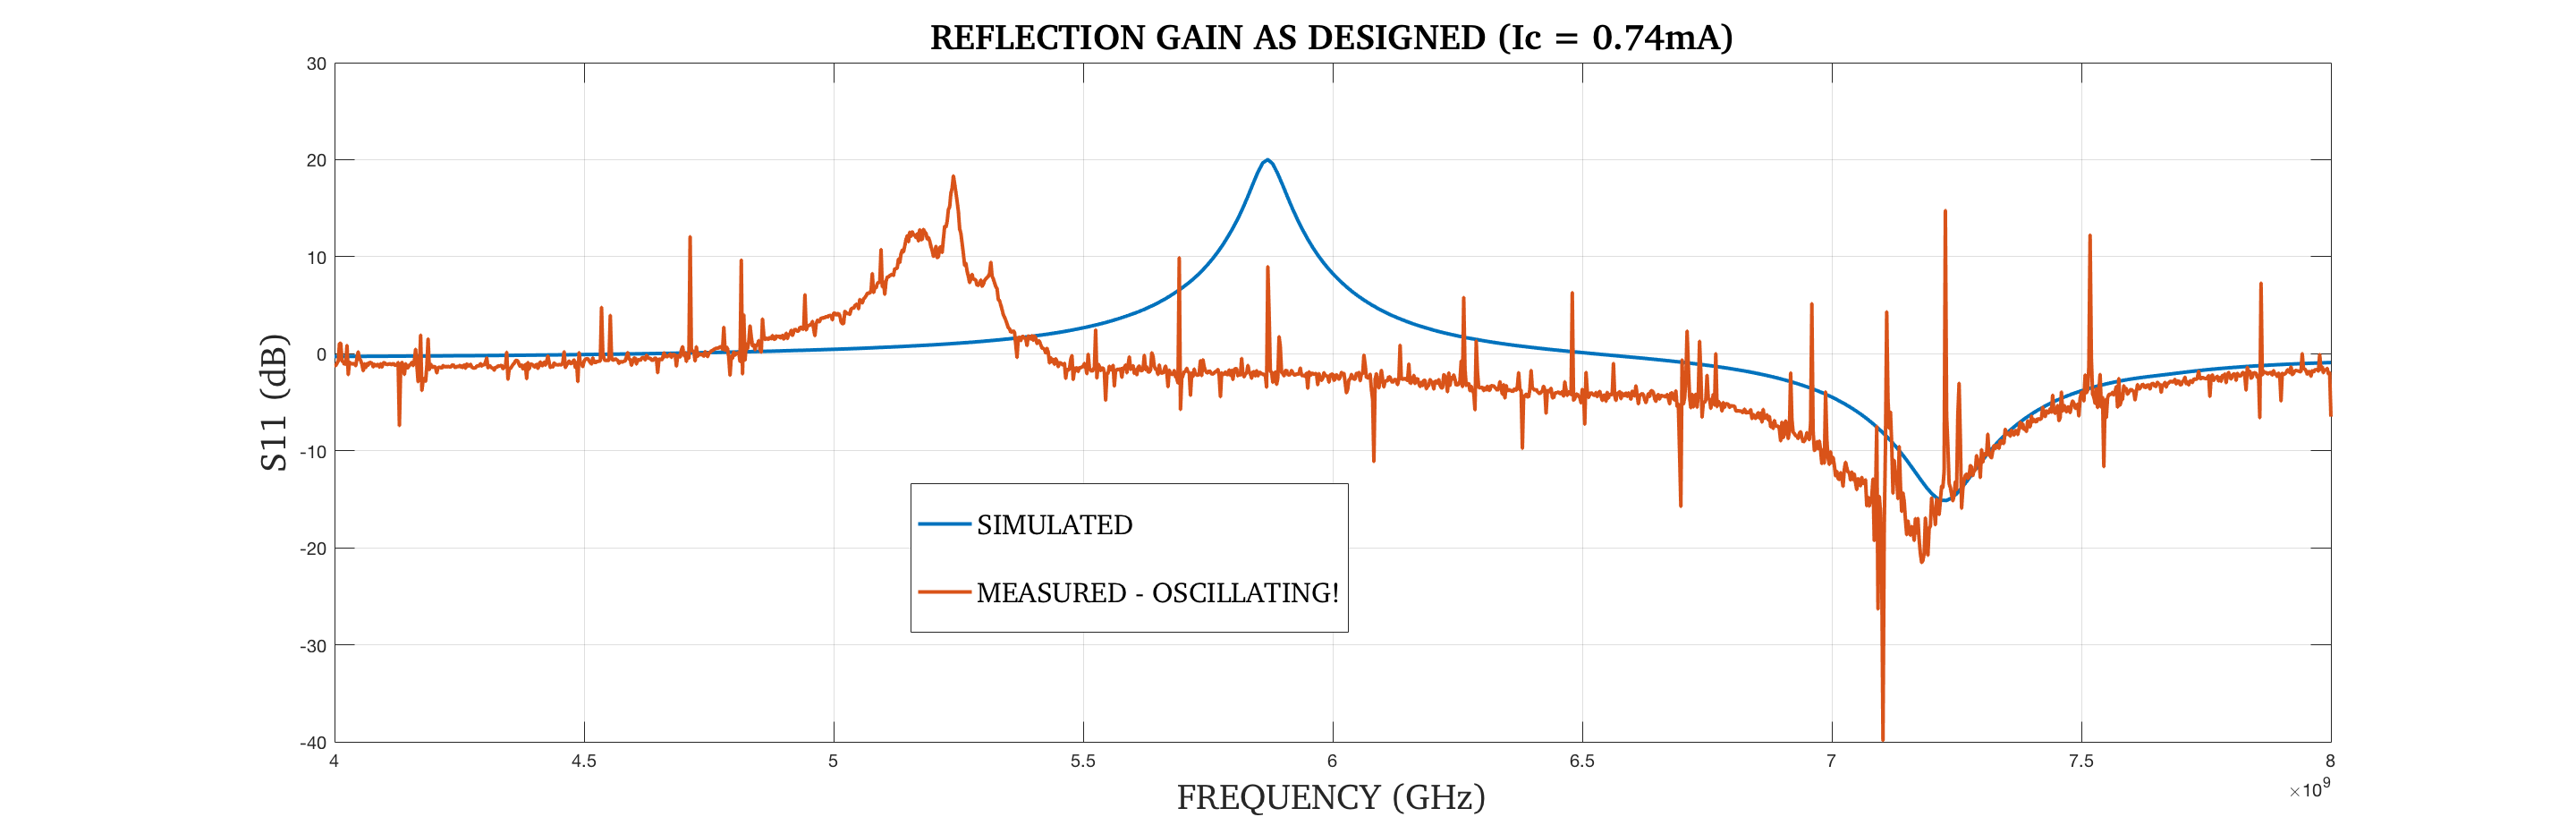
\includegraphics[width=1\textwidth] {Figures/S11_originalDesign.png}
  \caption{Simulated Vs Measured at Design Bias}
    \label{fig:f1}
\end{figure}

Clearly we can see that the design is oscillating when tested at the \textit{Design Bias}. When the bias current is
reduced we can remove the oscillation. A graph of the Measured vs Simulated at the \textit{Optimized Bias} is shown below.

\section{Results}
\begin{figure}[H]
  \centering
  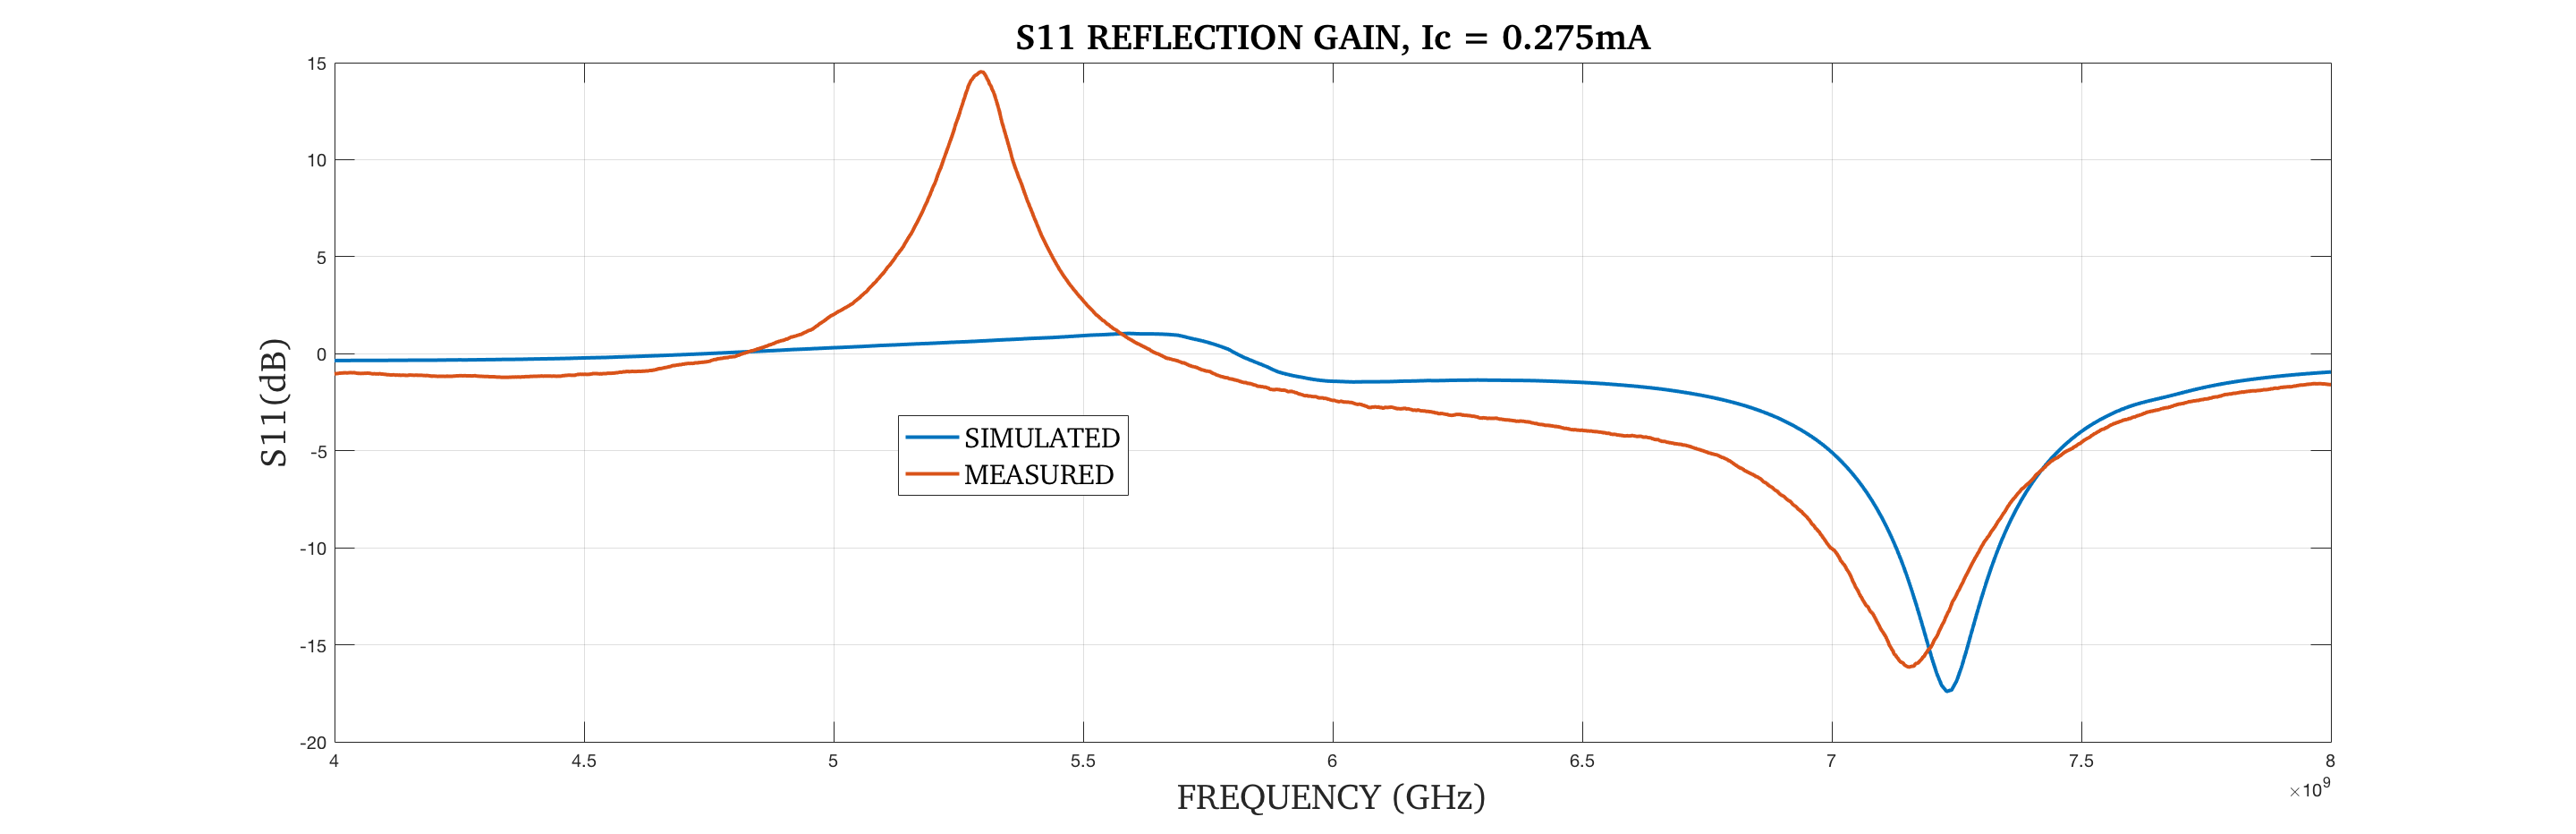
\includegraphics[width=1\textwidth] {Figures/S11_optimizedTest.png}
  \caption{Simulated Vs Measured at Optimized Bias}
    \label{fig:f2}
\end{figure}

The stability is confirmed by attaching the amplifier to a spectrum analyzer. To understand why the frequency
is shifted and why a different bias condition is required for stability we must analyze the impedance parameters.

\section{Comparison of Impedance Parameters}
\subsection{Unpowered Analysis}
  First let's take a look at the magnitude plot of the input when the transistor is unpowered and then break it down to it's
  input impedance
  \begin{figure}[H]
    \centering
    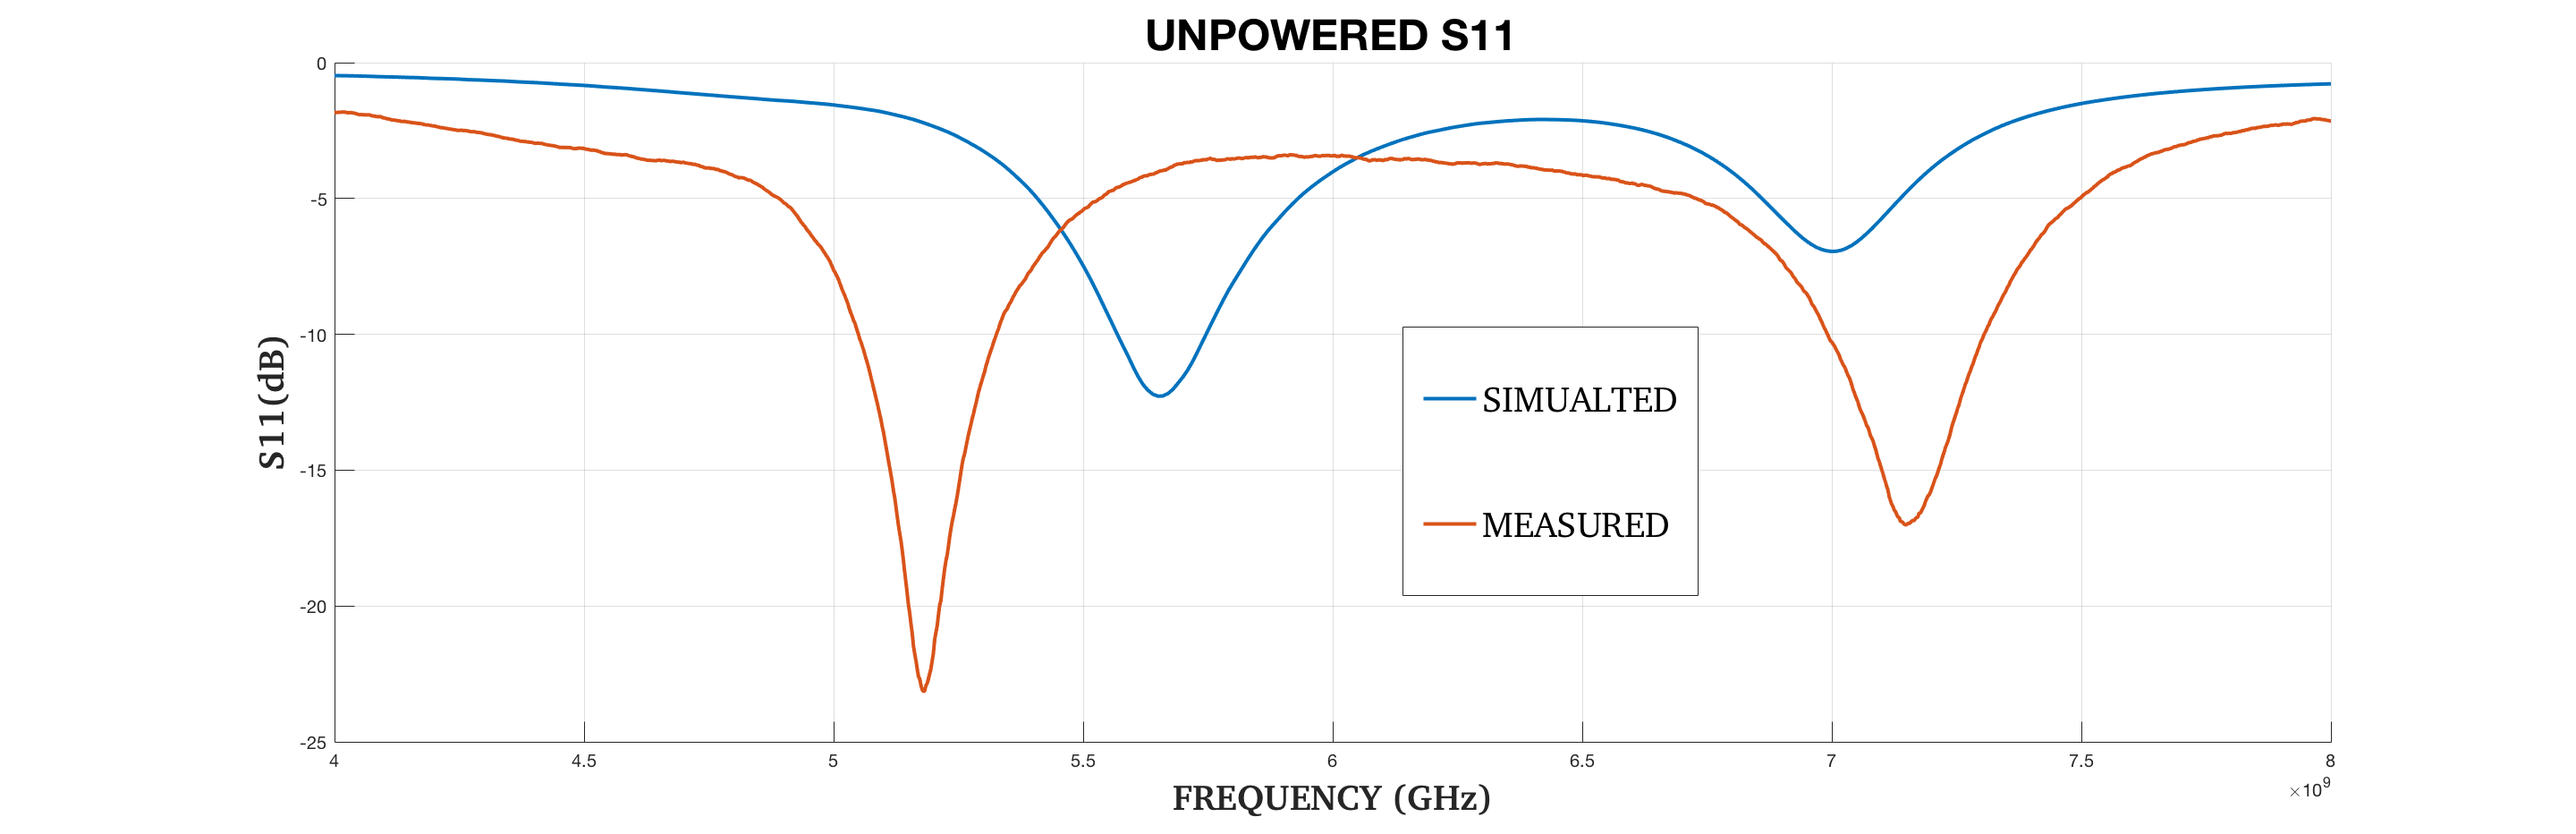
\includegraphics[width=1\textwidth] {Figures/unpowered_s11.png}
    \caption{Unpowered S11 Magnitude (dB)}
      \label{fig:f3}
  \end{figure}

  \begin{figure}[H]
    \centering
    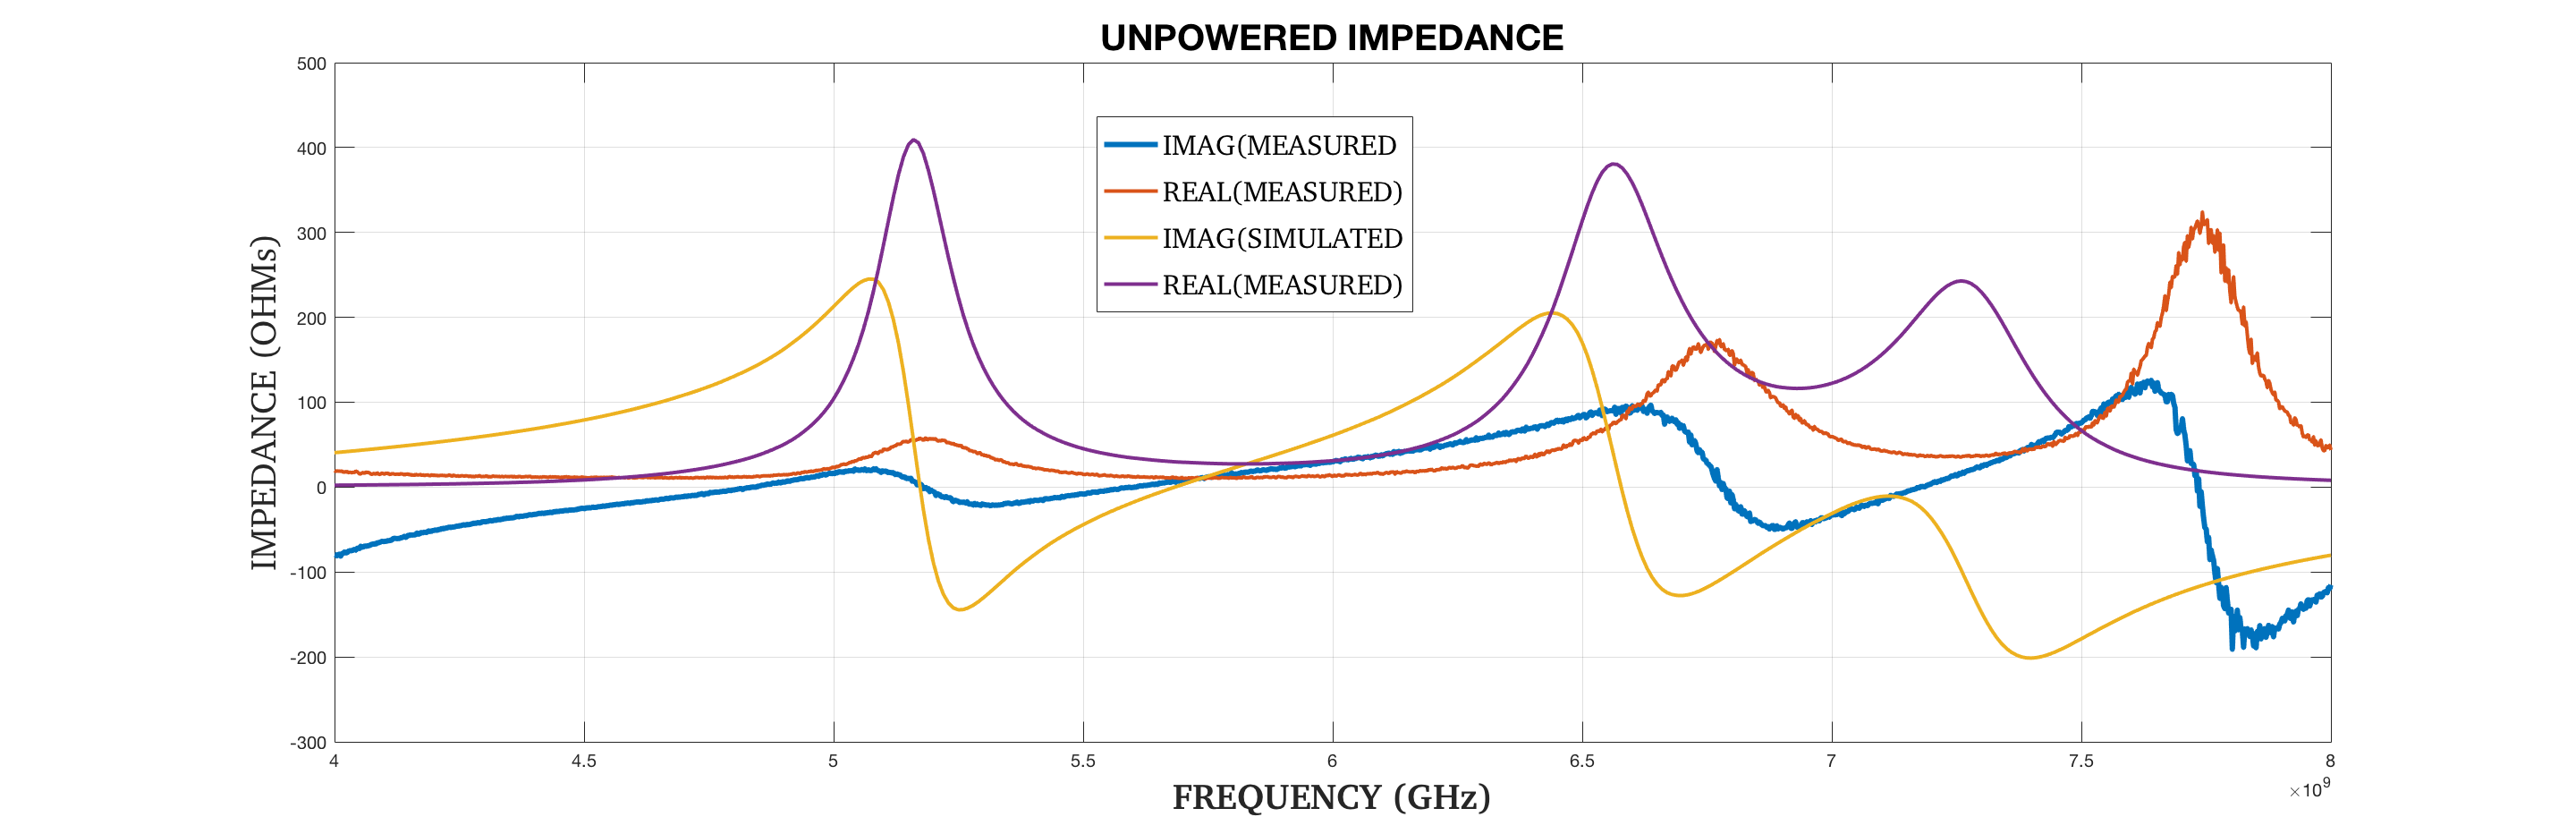
\includegraphics[width=1\textwidth] {Figures/unpowered_impedance.png}
    \caption{Unpowered Real and Imaginary Impedances}
      \label{fig:f4}
  \end{figure}

In the area of interest (5-6GHz) it is see that the input is considerably more capacitive in the measured case. This
results in a lower Q at the resonance. We will see if the same phenomena is present in the powered case. (\textbf{NEXT PAGE})
\clearpage
\subsection{Powered at Optimized Bias}
\begin{figure}[H]
  \centering
  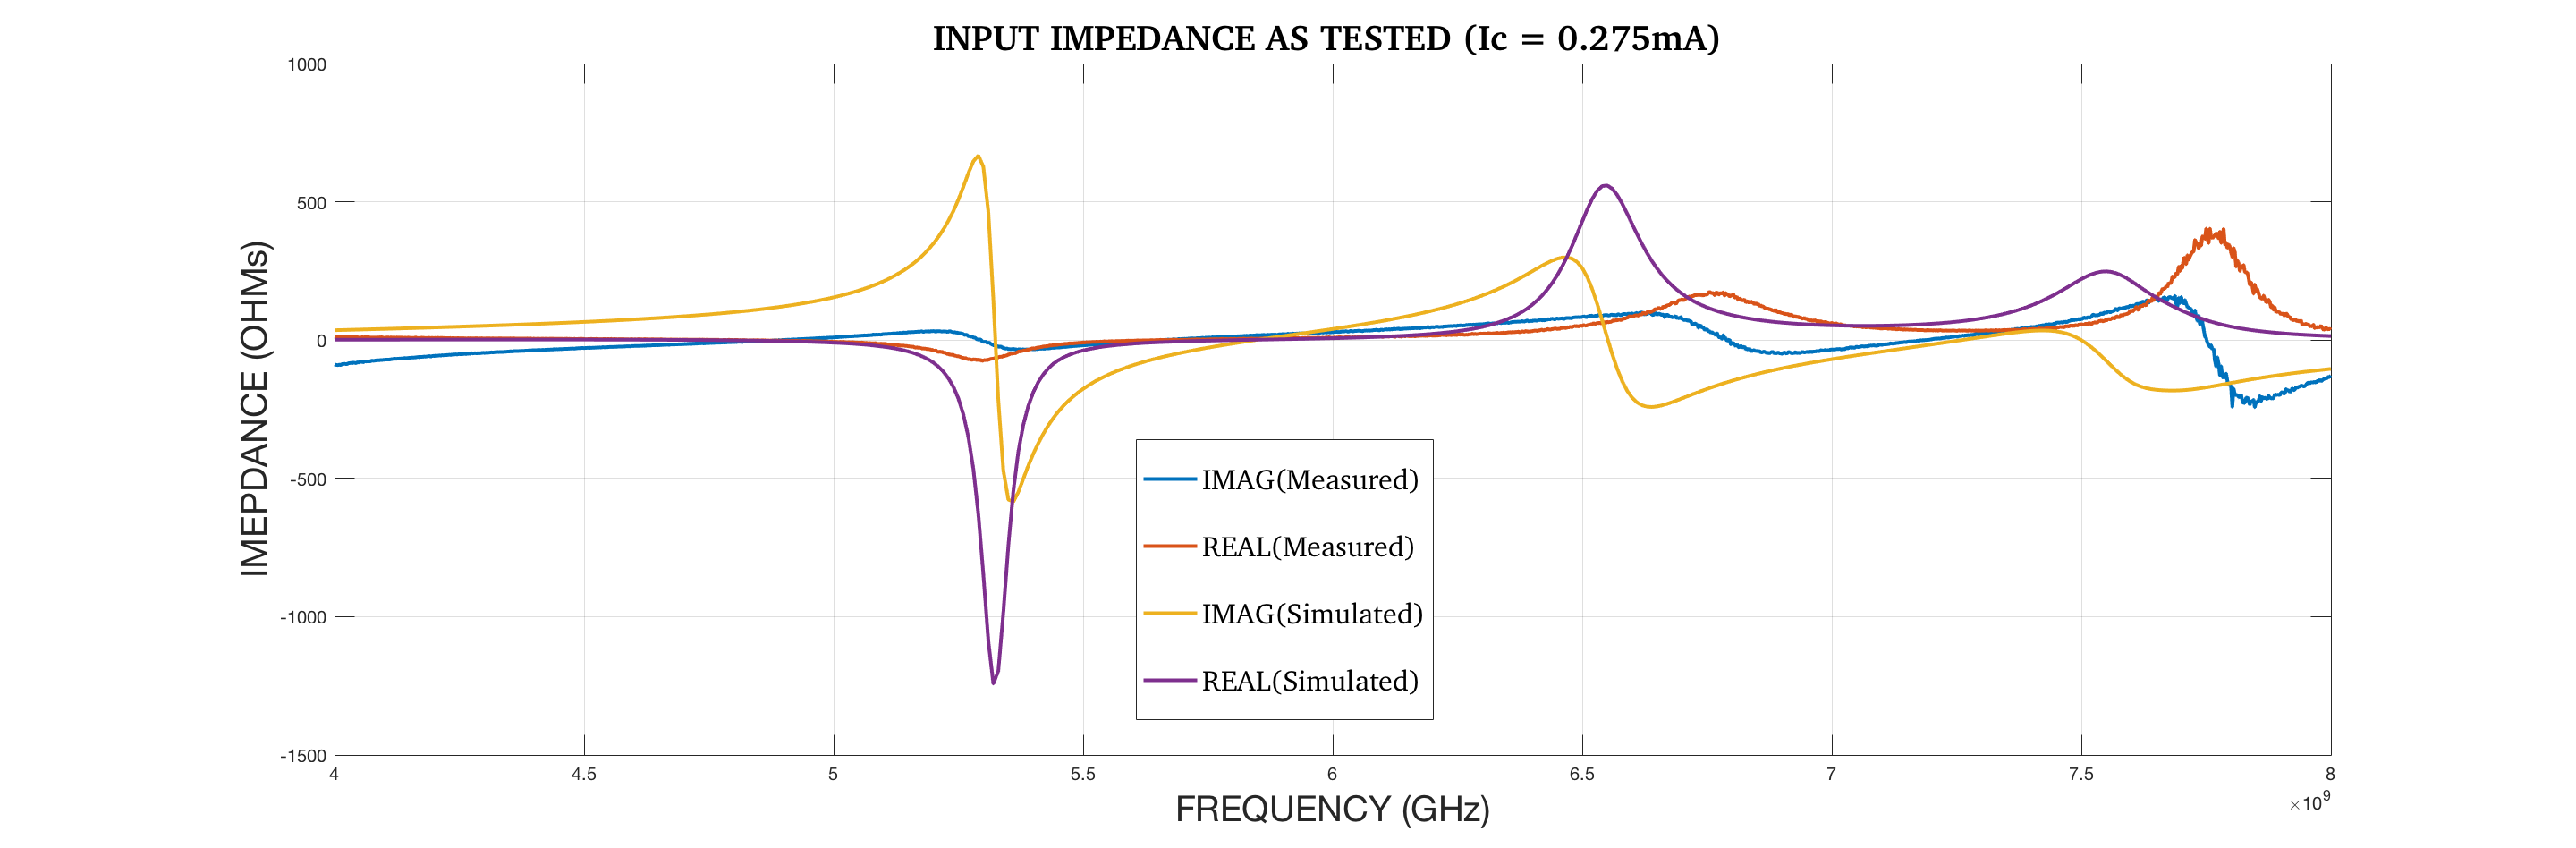
\includegraphics[width=1\textwidth] {Figures/Impedance_optimizedTest.png}
  \caption{Powered Real and Imaginary Impedances at Optimized Bias}
    \label{fig:f5}
\end{figure}

It can be see that the resonant frequency in the negative resistance region is the same for both simulated and measured. However the
magnitude is different. Again it is clear that the imaginary component has been shifted capacitively (bizarre). This explains why both the frequency
is shifted and why it will oscillate at the \textit{Design Bias}. I will elaborate... \\

\vspace{2mm}We know from negative conductor theory that the magnitude is inversely proportional to transistor $g_m$ therefore
the value of the negative resistance (seen as the dip in Figure ~\ref{fig:f5}) will increase as the bias current is decreased.
We also know from negative conductor theory that oscillation occurs at $|G_{IN}(0,\omega)| > G_L(\omega)$. Therefore as we reduce the
bias current $|G_{IN}(0,\omega)|$ is also reduced and oscillations are removed. The shift in frequency with respect to the S11 Magnitude plot
is also easily explained by observing these impedance parameters. Since the $ Q $ of the circuit is different the frequency at which the
resistance looks close to $ 50 \Omega$ is slightly different.\\

\vspace{3mm} I think it will be helpful for us to have a conversation about the design and theory of the circuit. That'll probably help
reveal what is going on.
\clearpage
%\begin{figure}[H]
%  \centering
%  \includegraphics[width=1\textwidth] {Figures/circuit_noMicrostrip.png}
%  \caption{Reflection Amplifier Schematic}
%    \label{fig:f3}
%\end{figure}

%\begin{table}[H]
%\centering
% \begin{tabular}{ | c | c |}
   %\hline
    %\textbf{Final Values} & \textbf{Manufacturer and PN}\\
    %\hline
    %\hline
    %$8.2nH$ & Johanson Tech JTI\_L-14C8N2\_SER \\
    %\hline
  %\end{tabular}
  %\caption{Final BOM}
  %\label{table:finalvals}
%\end{table}
%----------------------------------------------------------------------------------------
%	REFERENCES
%----------------------------------------------------------------------------------------
%\section{References}
%\printbibliography[heading=none]
%\newpage
%----------------------------------------------------------------------------------------
%	APPENDIX
%---------------------------------------------------------------------------------------
\begin{appendices}
\section{Meeting Agenda}
\begin{itemize}
  \item First let's take a look at the magnitude plot for 3 different tested units and the executive summary
  \item Review operation of transistor circuit
  \item Discuss Executive Summary
  \item Impedance plot powered showing change in Q
  \item Impedance plot unpowered with extended frequency range showing additional resonance.
  \item Appears more lossy... thoughts????

  \item Moving forward... thesis goals.
  \item Rotman lens design... retrodirectivity + analysis of radar cross section of system

  \item TIME FOR SEMINAR?
\end{itemize}

\end{appendices}

\end{document}
